\documentclass{standalone}

\usepackage{amsmath}
\usepackage{tikz}
\usetikzlibrary{circuits.ee.IEC}
\usepackage{placeins}

\begin{document}
	


	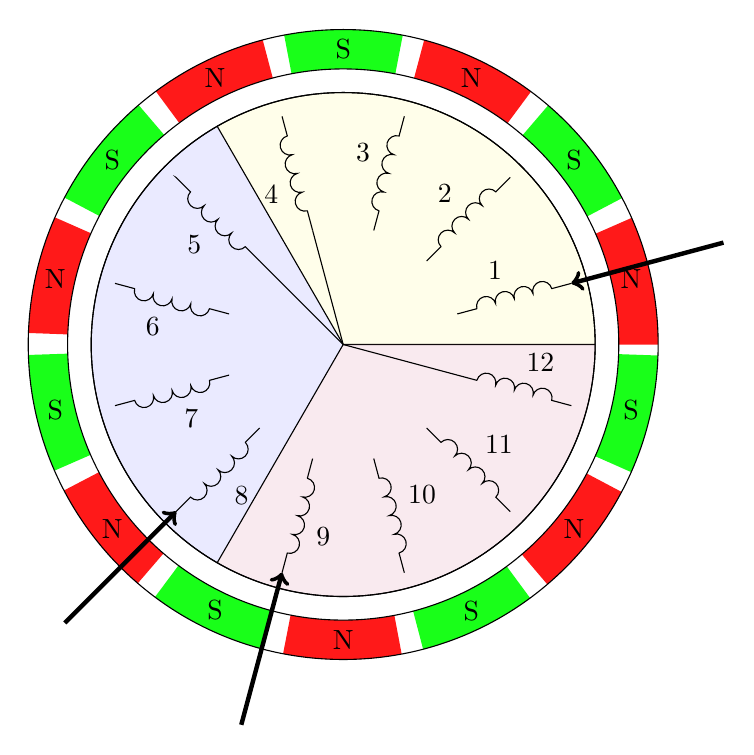
\begin{tikzpicture}[
		point/.style={circle,draw,minimum size=#1},
		point/.default=0pt,
		circuit ee IEC]
		
		
		
		%rotor
		
		\foreach \anfang/\ende/\farbe in { 0/23.7/red!90, 27.7/49.4/green!90,  53.4/75.1/red!90, 79.1/100.8/green!90,  104.8/126.5/red!90, 130.5/152.2/green!90, 156.2/177.9/red!90, 
			181.9/203.6/green!90,  207.6/229.3/red!90, 233.3/255/green!90!,  259/280.7/red!90, 284.7/306.4/green!90,  310.4/332.1/red!90, 336.1/358/green!90}
		\draw[fill=\farbe,draw=none] (0,0) -- (\anfang:4cm) arc (\anfang:\ende:4cm);
		
		\draw[fill=white,draw=none] (0,0) circle (3.5cm);
		
		\foreach[count=\i,evaluate=\i as \angle using (\i-1)*(360/14)+12.85] \text in {N,S,N,S,N,S,N,S,N,S,N,S,N,S}
		\node (node\i) at (\angle:3.75) {\text};
		
		%stator
		%spulen zuordnung
		\begin{scope}[fill opacity=0.1]
		\foreach \anfang/\ende/\farbe in {0/120/yellow!40!white, 120/240/blue!40!white, 240/360/purple!40!white}
		\draw[draw=black, fill=\farbe, fill opacity=0.2] (0,0) -- (\anfang:3.2cm) arc (\anfang:\ende:3.2cm);
		\end{scope}
		
		%spulen
		\foreach[count=\i,evaluate=\i as \angle using (\i-1)*(360/12)+15] \text in {1,2,3,4,5,6,7,8,9,10,11,12}
		\draw ({cos(\angle)*1.5},{sin(\angle)*1.5}) to [inductor={info={\text}}] ({cos(\angle)*3},{sin(\angle)*3});
		
		
		%spulenverbindung große spulen
		\foreach \angle in {(4-1)*(360/12)+15, (5-1)*(360/12)+15, (12-1)*(360/12)+15}	
		\draw (0,0) to ({cos(\angle)*1.5},{sin(\angle)*1.5});
		
		
		%anschlüsse
		\foreach \angle in {(1-1)*(360/12)+15, (8-1)*(360/12)+15, (9-1)*(360/12)+15}	
		\draw[ultra thick, ->] ({cos(\angle)*5},{sin(\angle)*5}) to ({cos(\angle)*3},{sin(\angle)*3});	
		
		
		
		
		%ränder	
		\draw (0,0) circle [radius=3.2cm];
		\draw (0,0) circle [radius=3.5cm];
		\draw (0,0) circle [radius=4cm];
		
		
	\end{tikzpicture}


\end{document}